\section{Methodology}
\label{sec:methods}

\subsection{Dataset}
\label{subsec:dataset}

The data



\subsection{Preprocessing}
\label{subsec:prepro}
The proposed automatic preprocessing steps for the MRIs consist of:
bias correction using the N4ITK algorithm \cite{n4itk}, 
image normalization to an interval of [0,1],
automatic selection of a region of interest (ROI), 
image re-sampling to a resolution of $0.5 \times 0.5 \times 0.5$ mm, 
and contour interpolation using optical flow.

The method for selecting a ROI from multiple MRI planes was originally proposed in \cite{anneke}, and consists of reducing the size of the MRIs 
(axial, sagittal, and coronal)
by the intersection of its three corresponding rectangular prisms. Resampling
of the images is performed using linear interpolation with the ITK software \cite{itk}. 

Manual contours made by the experts were carried on the original MRI
resolutions and not on the higher resolution version; therefore, 
the necessity for interpolating them. 
The proposed interpolation is performed in two dimensions, and
is computed independently between every two consecutive slices of the contour. First, optical flow is obtained between the two contours using the  
Farneback method. Then, the contours are interpolated linearly following
the directions of the optical flow. Figure \ref{fig:of1} shows an
example of the resulting interpolated contour using this method. 
\begin{figure}[h]
    \centering
    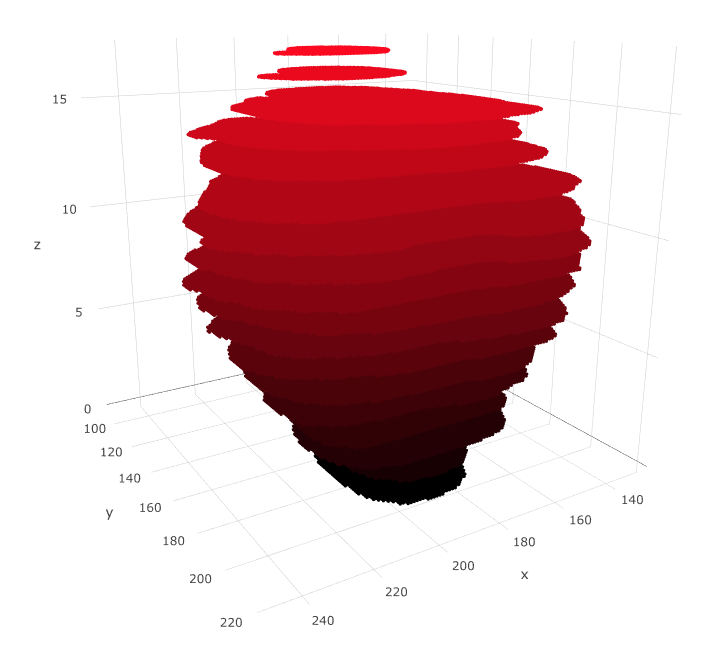
\includegraphics[totalheight=.15\textheight]{imgs/methodology/OF_1.png}
    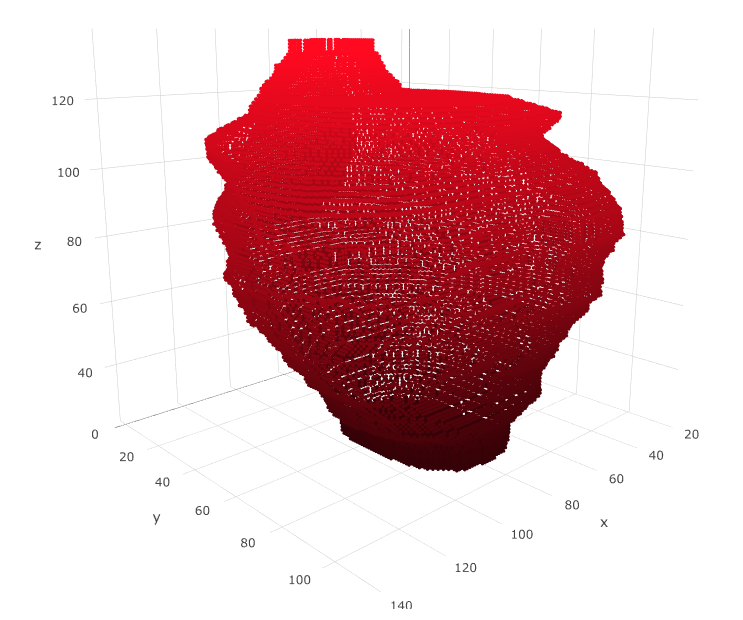
\includegraphics[totalheight=.15\textheight]{imgs/methodology/OF_2.png}
    \caption{Contours provided by experts are interpolated using optical flow and
    linear interpolation. On the left:
    original contours with 17 slices. On the right: interpolated contours with 68 slices.}
    \label{fig:of1}
\end{figure}

\subsection{Proposed architecture}
The proposed CNN consist of a 3D multistream architecture that follows the analysis
and synthesis path of the 3D U-Net \cite{cciccek20163d}. The input of each stream is
the postprocessed ROI for one of three MRI scans (axial, sagittal, and coronal),
with a resolution of $168^3$. During the analysis phase, a combination
of two convolutional layers and one max pool layer is applied three times. The second 
convolutional layer in each set doubles the number of channels. 
In the synthesis phase, a similar set of two convolutional layers and
one deconvolution is applied, followed by batch normalization.
Figure \ref{fig:nn} shows the proposed model, where 
all convolutional layers use a filter size of $3 \times 3 \times 3$ and
rectified linear unit (ReLu) as the activation function; with the exception
of the last layer which uses a filter size of $1 \times 1 \times 1$  and Sigmoid
as the activation function. 
\begin{figure*}[h]
    \centering
    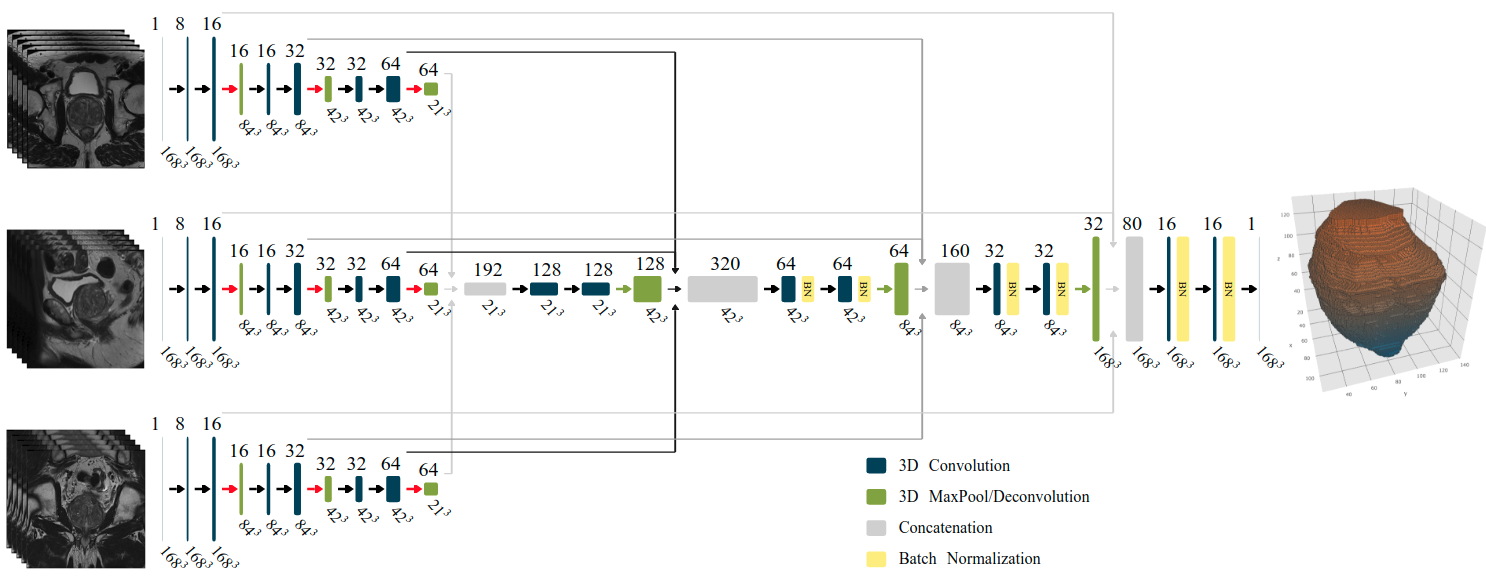
\includegraphics[totalheight=.275\textheight]{imgs/methodology/NN.png}
    \caption{Multistream 3D convolutional network architecture. The input of the network
    are $168^3$ volumes from the MRI planes: axial, sagittal, and coronal. }
    \label{fig:nn}
\end{figure*}

With the proposed architecture the training time is reduced in half, compared
to the original architecture of Meyer et al. \cite{anneke}. The performance
improvement is obtained by reducing the number of filters 
from 192 to 128 in the last layer of the analysis path, and
by adding batch normalization after every convolutional layer 
in the synthesis path.

\subsection{Training}
\label{subsec:training}
The selected optimization algorithm is Stochastic Gradient Descent (SGD) with a
learning rate $\alpha = 0.05$, momentum of 0.2 and decay of $10^{-7}$. The training is performed
for 1000 epochs, a batch size of 50, and an early stop mechanism for the validation
loss if not improved by $\delta = 0.001$ after 70 iterations. 

The loss function used for the training is the negative Dice Similarity Coefficient (DSC):
\begin{equation}
\text{Loss} = \frac{2 \sum_{i=1}^{N}p_it_i}{\sum_{i=1}^{N}p_i^2 + \sum_{i=1}^{N}t_i^2 + \varepsilon} 
\label{eq:dsc}
\end{equation}
%where N is the total number of voxels in the image, when training for prostate segmenation,
%and the number of voxels \textbf{inside} the prostate, when training for the PZ. The segmentation
%of the PZ assumes that we already know where the prostate is, so we do not take into
%account anything outside the prostate for the loss function. 
where N is the total number of voxels in the image, $p_i$ the voxel values for the 
prediction of the network, and $t_i$ the true voxel values of the prostate or PZ masks.

The dataset was split into 90\% for training and 10\% for
validation. Also, in order to compare the robustness of the models with respect to changes
in MRI vendor machines,  a distinct model was trained for each dataset: GE (n=100), 
Siemens (n=328), combined model (n=428). 

To analyze how 3D data augmentation can influence the sensitivity of the models
against different vendor machines, additional models were trained 
incorporating data augmentation. The data augmentation is performed by flipping the
images in the sagittal axis,  shifting in any direction up to 10\% of the image size, and
blurring the images using Gaussian blur up to $\sigma = 3$. Each data augmentation
method is applied with a random chance of $1/3$.

A total number of 12 models were trained from the combination of 
three datasets, using or not data augmentation, and training for the segmentation 
of the prostate or the PZ. 
